\chapter{Жолды өңдеу алгоритмдері}

Бұл тарауда жолдарды тиімді өңдейтін алгоритмдер
қарастырылады. Жолға байланысты көптеген мәселелерді
$O(n^2)$ уақытта шешуге  болады, бірақ 
$O(n)$ немесе $O(n \log n)$ уақытта жұмыс істейтін
алгоритмдерді табу қиынырақ болады. 


% This chapter deals with efficient algorithms
% for string processing.
% Many string problems can be easily solved
% in $O(n^2)$ time, but the challenge is to
% find algorithms that work in $O(n)$ or $O(n \log n)$
% time.

\index{үлгімен салғастыру}

Мысалы жолды өңдейтін негізгі есептердің бірі 
-- \key{үлгімен салғастыру} есебі. Бізге ұзындығы 
$n$ болатын жол берілген және ұзындығы $m$ болатын
үлгі берілген. Біздің тапсырмамыз -- берілген жолда 
қанша рет үлгі кездесетінін табу.
Мысалы егер үлгі \texttt{ABC} болса, ол 
\texttt{ABABCBABC} жолында 2 мәрте кездеседі. 

% For example, a fundamental string processing
% problem is the \key{pattern matching} problem:
% given a string of length $n$ and a pattern of length $m$,
% our task is to find the occurrences of the pattern
% in the string.
% For example, the pattern \texttt{ABC} occurs two
% times in the string \texttt{ABABCBABC}.

Үлгімен салғастыру есебі 
жолдың барлық позицияларын үлгімен басталуына тексеретін
толық ізденіс алгоритмі арқылы $O(nm)$ уақытта жеңіл 
шығарылады. Дегенмен бұл тарауда тек $O(n+m)$ уақыт
қажет ететін тиімдірек алгоритмдер бар екенін көреміз.

% The pattern matching problem can be easily solved
% in $O(nm)$ time by a brute force algorithm that
% tests all positions where the pattern may
% occur in the string.
% However, in this chapter, we will see that there
% are more efficient algorithms that require only
% $O(n+m)$ time.

\index{жол}

\section{Жол терминологиясы}

\index{әліпби}

Бүкіл тарау бойынша жолды нөлмен индекстейтін боламыз. 
Демек ұзындығы $n$ болатын жол 
$\texttt{s}[0],\texttt{s}[1],\ldots,\texttt{s}[n-1]$
таңбалардан тұрады. Жолда кездесе алатын 
таңбалардың жиынтығы \key{әліпби} деп аталады.
Мысалы 
$\{\texttt{A},\texttt{B},\ldots,\texttt{Z}\}$
әліпбиі ағылшын бас әріптерінен тұрады. 

% Throughout the chapter, we assume that
% zero-based indexing is used in strings.
% Thus, a string \texttt{s} of length $n$
% consists of characters
% $\texttt{s}[0],\texttt{s}[1],\ldots,\texttt{s}[n-1]$.
% The set of characters that may appear
% in strings is called an \key{alphabet}.
% For example, the alphabet
% $\{\texttt{A},\texttt{B},\ldots,\texttt{Z}\}$
% consists of the capital letters of English.

\index{ішжол}

\key{Ішжол} -- жолдың қатар келетін әріптер тізбегі.
Біз $\texttt{s}[a \ldots b]$ нотациясын 
$a$-дан басталатын $b$-дан бітетін ішжолға 
қолданатын боламыз. Ұзындығы $n$ болатын 
жолда $n(n+1)/2$ ішжол бар. Мысалы, \texttt{ABCD} жолының
ішжолдары -- \texttt{A}, \texttt{B}, \texttt{C}, \texttt{D},
\texttt{AB}, \texttt{BC}, \texttt{CD},
\texttt{ABC}, \texttt{BCD} және \texttt{ABCD}.

% A \key{substring} is a sequence of consecutive
% characters in a string.
% We use the notation $\texttt{s}[a \ldots b]$
% to refer to a substring of \texttt{s}
% that begins at position $a$ and ends at position $b$.
% A string of length $n$ has $n(n+1)/2$ substrings.
% For example, the substrings of
% \texttt{ABCD} are
% \texttt{A}, \texttt{B}, \texttt{C}, \texttt{D},
% \texttt{AB}, \texttt{BC}, \texttt{CD},
% \texttt{ABC}, \texttt{BCD} and \texttt{ABCD}.

\index{іштізбек}


\key{Іштізбек} деп тізбектегі кейбір элементтерді алып тастай отырып, бірақ қалған элементтердің орналасу тәртібін өзгертпестен жасауға болатын тізбекті айтамыз. 
Ұзындығы $n$ болатын жолда $2^n-1$ іштізбек бар.
Мысалы, \texttt{ABCD} жолдың іштізбектері --
\texttt{A}, \texttt{B}, \texttt{C}, \texttt{D},
\texttt{AB}, \texttt{AC}, \texttt{AD},
\texttt{BC}, \texttt{BD}, \texttt{CD},
\texttt{ABC}, \texttt{ABD}, \texttt{ACD},
\texttt{BCD} және \texttt{ABCD}.

% A \key{subsequence} is a sequence of
% (not necessarily consecutive) characters
% in a string in their original order.
% A string of length $n$ has $2^n-1$ subsequences.
% For example, the subsequences of
% \texttt{ABCD} are
% \texttt{A}, \texttt{B}, \texttt{C}, \texttt{D},
% \texttt{AB}, \texttt{AC}, \texttt{AD},
% \texttt{BC}, \texttt{BD}, \texttt{CD},
% \texttt{ABC}, \texttt{ABD}, \texttt{ACD},
% \texttt{BCD} and \texttt{ABCD}.

\index{префикс}
\index{суффикс}

\key{Префикс} -- жолдың басынан басталатын ішжол, ал 
\key{суффикс} -- жолдың соңында аяқталатын ішжол. 
Мысалы, \texttt{ABCD} жолының префикстері --
\texttt{A}, \texttt{AB}, \texttt{ABC} және \texttt{ABCD}. Ал
суффикстері -- \texttt{D}, \texttt{CD}, \texttt{BCD} және \texttt{ABCD}.

% A \key{prefix} is a substring that starts at the beginning
% of a string,
% and a \key{suffix} is a substring that ends at the end
% of a string.
% For example,
% the prefixes of \texttt{ABCD} are
% \texttt{A}, \texttt{AB}, \texttt{ABC} and \texttt{ABCD},
% and the suffixes of \texttt{ABCD} are
% \texttt{D}, \texttt{CD}, \texttt{BCD} and \texttt{ABCD}.

\index{айналым}

\key{Айналым} жолдың басындағы таңбаларды бір-бірден соңына 
жылжыту (немесе керісінше) арқылы өңдіріледі. 
Мысалы, \texttt{ABCD} жолының айналымдары -- 
\texttt{ABCD}, \texttt{BCDA}, \texttt{CDAB} және \texttt{DABC}.

% A \key{rotation} can be generated by moving
% the characters of a string one by one from the beginning
% to the end (or vice versa).
% For example, the rotations of \texttt{ABCD} are
% \texttt{ABCD}, \texttt{BCDA}, \texttt{CDAB} and \texttt{DABC}.

\index{период}

Период -- өзін қайталау арқылы жолды құрастыруға болатын
жолдың префиксі. Соңғы қайталау толық болмауы мүмкін,
яғни соңғы қайталау периодтың префиксы болуы мүмкін. 
Мысалы, \texttt{ABCABCA} жолының ең қысқа периоды \texttt{ABC}.

% A \key{period} is a prefix of a string such that
% the string can be constructed by repeating the period.
% The last repetition may be partial and contain
% only a prefix of the period.
% For example, the shortest period of
% \texttt{ABCABCA} is \texttt{ABC}.

\index{шек}

Шек -- жолдың префиксі және суффиксі болатын
жол. Мысалы, \texttt{ABACABA} жолының шектері --
\texttt{A}, \texttt{ABA} және \texttt{ABACABA}.

% A \key{border} is a string that is both
% a prefix and a suffix of a string.
% For example, the borders of \texttt{ABACABA}
% are \texttt{A}, \texttt{ABA} and \texttt{ABACABA}.

\index{лексикографикалық рет}

Қарапайым тілмен айтқанда, \key{лексикографиялық реттілік} -- сөздердің сөздіктерде берілу реттілігі. Ресми анықтамасы мынадай: егер $p_i < q_i$ болатын $i$ позициясы болса және барлығы үшін j < i, $p_j = q_j$ болса, онда $p$ жолы лексикографиялық тұрғыдан $q$ жолынан кіші болады. Егер мұндай $i$ позициясы болмаса, $p$ ұзындығы $q$ ұзындығынан кем болған жағдайда $p$ лексикографиялық тұрғыдан $q$ ұзындығынан кіші болады. Мысалы, $abdc < abe$ және $abc < abcd$, мұндағы $p$ ұзындығы $q$-дан лексикографиялық тұрғыдан кіші болса, $p < q$ деп жазамыз.

% Strings are compared using the \key{lexicographical order}
% (which corresponds to the alphabetical order).
% It means that $x<y$ if either $x \neq y$ and $x$ is a prefix of $y$,
% or there is a position $k$ such that
% $x[i]=y[i]$ when $i<k$ and $x[k]<y[k]$.

\section{Префикс дарағы}

\index{префикс дарағы}

\key{Префикс дарағы} -- жолдардың
жиынын қолдайтын түбірлі дарақ. 
Жиынның әрбір жолы түбірден 
басталатын таңбалар тізбегі ретінде сақталады.
Егер екі жолдың ортақ префиксі болса, олар дарақта да ортақ тізбекке ие болады.

% A \key{trie} is a rooted tree that
% maintains a set of strings.
% Each string in the set is stored as
% a chain of characters that starts at the root.
% If two strings have a common prefix,
% they also have a common chain in the tree.

Мысалға келесі префикс дарағын қарастырайық:
% For example, consider the following trie:

\begin{center}
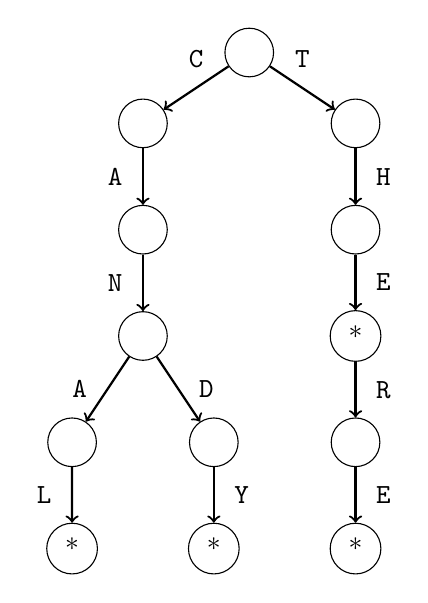
\begin{tikzpicture}[scale=0.9]
\node[draw, circle] (1) at (0,20) {$\phantom{1}$};
\node[draw, circle] (2) at (-1.5,19) {$\phantom{1}$};
\node[draw, circle] (3) at (1.5,19) {$\phantom{1}$};
\node[draw, circle] (4) at (-1.5,17.5) {$\phantom{1}$};
\node[draw, circle] (5) at (-1.5,16) {$\phantom{1}$};
\node[draw, circle] (6) at (-2.5,14.5) {$\phantom{1}$};
\node[draw, circle] (7) at (-0.5,14.5) {$\phantom{1}$};
\node[draw, circle] (8) at (-2.5,13) {*};
\node[draw, circle] (9) at (-0.5,13) {*};
\node[draw, circle] (10) at (1.5,17.5) {$\phantom{1}$};
\node[draw, circle] (11) at (1.5,16) {*};
\node[draw, circle] (12) at (1.5,14.5) {$\phantom{1}$};
\node[draw, circle] (13) at (1.5,13) {*};

\path[draw,thick,->] (1) -- node[font=\small,label=\texttt{C}] {} (2);
\path[draw,thick,->] (1) -- node[font=\small,label=\texttt{T}] {} (3);
\path[draw,thick,->] (2) -- node[font=\small,label=left:\texttt{A}] {} (4);
\path[draw,thick,->] (4) -- node[font=\small,label=left:\texttt{N}] {} (5);
\path[draw,thick,->] (5) -- node[font=\small,label=left:\texttt{A}] {} (6);
\path[draw,thick,->] (5) -- node[font=\small,label=right:\texttt{D}] {} (7);
\path[draw,thick,->] (6) -- node[font=\small,label=left:\texttt{L}] {}(8);
\path[draw,thick,->] (7) -- node[font=\small,label=right:\texttt{Y}] {} (9);
\path[draw,thick,->] (3) -- node[font=\small,label=right:\texttt{H}] {} (10);
\path[draw,thick,->] (10) -- node[font=\small,label=right:\texttt{E}] {} (11);
\path[draw,thick,->] (11) -- node[font=\small,label=right:\texttt{R}] {} (12);
\path[draw,thick,->] (12) -- node[font=\small,label=right:\texttt{E}] {} (13);
\end{tikzpicture}
\end{center}

Бұл дарақ 
$\{\texttt{CANAL},\texttt{CANDY},\texttt{THE},\texttt{THERE}\}$ жиынына
сәйкес. Төбедегі * таңбасы жиынның 
бір жолы осы төбеде аяқталатынын көрсетеді.
Ондай таңба қажет-ақ, өйткені бір жол екінші 
жолдың префиксі болуы мүмкін. Мысалы, жоғарыдағы 
префикс дарағында \texttt{THE} жолы \texttt{THERE} жолының
префиксі болады.

% This trie corresponds to the set
% $\{\texttt{CANAL},\texttt{CANDY},\texttt{THE},\texttt{THERE}\}$.
% The character * in a node means that
% a string in the set ends at the node.
% Such a character is needed, because a string
% may be a prefix of another string.
% For example, in the above trie, \texttt{THE}
% is a prefix of \texttt{THERE}.

Ұзындығы $n$ болатын жолдың дарақта бар-жоғын
$O(n)$ уақытта тексере аламыз, өйткені біз
түбір төбеден басталатын тізбек бойынша ере аламыз.
Сондай-ақ ұзындығы $n$ болатын жолды 
басында тізбек бойынша ере отырып, кейін қажеттілігіне қарай дараққа жаңа төбелерді
тіркей отырып, $O(n)$ уақытта дараққа қоса аламыз. 

% We can check in $O(n)$ time whether a trie
% contains a string of length $n$,
% because we can follow the chain that starts at the root node.
% We can also add a string of length $n$ to the trie
% in $O(n)$ time by first following the chain
% and then adding new nodes to the trie if necessary.


Префикс дарағын қолдана отырып, берілген жолдың жиымға жататын ең ұзын префиксін таба аламыз. 
Сондай-ақ, әр төбеде қосымша ақпаратты сақтай отырып, біз
жиынға жататын және префиксі берілген жол болатын 
жолдар санын есептей аламыз.

% Using a trie, we can find
% the longest prefix of a given string
% such that the prefix belongs to the set.
% Moreover, by storing additional information
% in each node,
% we can calculate the number of
% strings that belong to the set and have a
% given string as a prefix.

Префикс дарағын келесі жиым ретінде сақтауға болады:
\begin{lstlisting}
int trie[N][A];
\end{lstlisting}
мұндағы $N$ -- төбелердің максималды саны
(жиындағы барлық жолдардың жиынтық ұзындығы)
және $A$ -- әліпбидің ұзындығы.
Префикс дарағындағы төбелер
$0,1,2,\ldots$ сандарымен нөмірленген. Түбірдің нөмірі -- 0 және
$\texttt{trie}[s][c]$ -- $s$ төбеден $c$ таңбасы арқылы
өткен кездегі тізбектегі келесі төбе. 

% The nodes of a trie are numbered
% $0,1,2,\ldots$ so that the number of the root is 0,
% and $\texttt{trie}[s][c]$ is the next node in the chain
% when we move from node $s$ using character $c$.

\section{Жол хэші}

\index{хэш}
\index{жол хеші}

\key{Жол хэші} арқылы екі жолдардың
тең екенін оңтайлы тексеруге болады.\footnote{Бұл әдіс Рабин-Карп үлгімен
салғастыру алгоритмінің арқасында танымал болды \cite{kar87}.} 
Идеясы жолдардың таңбаларын жекелеп тексерудің орнына
жолдардың хэштерін тексеруге негізделеді. 

% \key{String hashing} is a technique that
% allows us to efficiently check whether two
% strings are equal\footnote{The technique
% was popularized by the Karp–Rabin pattern matching
% algorithm \cite{kar87}.}.
% The idea in string hashing is to compare hash values of
% strings instead of their individual characters.

\subsubsection*{Хэшті есептеу}

\index{хэш}
\index{көпмүшелік хэш}

Жолдың \key{хэші} -- жолдың таңбалары арқылы 
есептелген сан. Егер жолдар бірдей болса,
олардың хэштері де бірдей болады. Демек 
бұл жолдардың хэші арқылы
жолдарды салыстыруға мүмкіндік береді.

% A \key{hash value} of a string is
% a number that is calculated from the characters
% of the string.
% If two strings are the same,
% their hash values are also the same,
% which makes it possible to compare strings
% based on their hash values.

Әдетте жолдың хэшін \key{көпмүшелік хэш} арқылы
есептейді. Ондай кезде ұзындығы $n$ болатын 
жолдың хэші 
\[(\texttt{s}[0] A^{n-1} + \texttt{s}[1] A^{n-2} + \cdots + \texttt{s}[n-1] A^0) \bmod B  ,\]
мұндағы $s[0],s[1],\ldots,s[n-1]$ -- \texttt{s} жолының таңбалар коды, %check
$A$ және $B$ -- алдын ала таңдалған тұрақтылар. 

% A usual way to implement string hashing
% is \key{polynomial hashing}, which means
% that the hash value of a string \texttt{s}
% of length $n$ is
% \[(\texttt{s}[0] A^{n-1} + \texttt{s}[1] A^{n-2} + \cdots + \texttt{s}[n-1] A^0) \bmod B  ,\]
% where $s[0],s[1],\ldots,s[n-1]$
% are interpreted as the codes of the characters of \texttt{s},
% and $A$ and $B$ are pre-chosen constants.

Мысалы, \texttt{ALLEY} жолы таңбаларының коды
келесідей:
% For example, the codes of the characters
% of \texttt{ALLEY} are:
\begin{center}
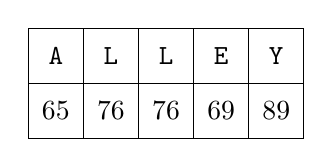
\begin{tikzpicture}[scale=0.7]
\draw (0,0) grid (5,2);

\node at (0.5, 1.5) {\texttt{A}};
\node at (1.5, 1.5) {\texttt{L}};
\node at (2.5, 1.5) {\texttt{L}};
\node at (3.5, 1.5) {\texttt{E}};
\node at (4.5, 1.5) {\texttt{Y}};

\node at (0.5, 0.5) {65};
\node at (1.5, 0.5) {76};
\node at (2.5, 0.5) {76};
\node at (3.5, 0.5) {69};
\node at (4.5, 0.5) {89};

\end{tikzpicture}
\end{center}

Демек егер $A=3$ және $B=97$ болса, \texttt{ALLEY} 
жолының хэші --
\[(65 \cdot 3^4 + 76 \cdot 3^3 + 76 \cdot 3^2 + 69 \cdot 3^1 + 89 \cdot 3^0) \bmod 97 = 52.\]

% Thus, if $A=3$ and $B=97$, the hash value
% of \texttt{ALLEY} is
% \[(65 \cdot 3^4 + 76 \cdot 3^3 + 76 \cdot 3^2 + 69 \cdot 3^1 + 89 \cdot 3^0) \bmod 97 = 52.\]

\subsubsection*{Алдын ала өңдеу}

Көпмүшелік хэш арқылы \texttt{s} жолының кез келген ішжолының хэшін
$O(n)$ уақыт алдын ала өңдеуден кейін $O(1)$ уақытта есептей аламыз. 
Идеясы $\texttt{h}[k]$ $\texttt{s}[0 \ldots k]$ префиксінің хэшінен тұратын \texttt{h} жиымын құруға негізделеді. 

% Using polynomial hashing, we can calculate the hash value of any substring
% of a string \texttt{s} in $O(1)$ time after an $O(n)$ time preprocessing.
% The idea is to construct an array \texttt{h} such that
% $\texttt{h}[k]$ contains the hash value of the prefix $\texttt{s}[0 \ldots k]$.
Жиынның мәндерін рекурсивті түрде келесі түрде есептеуімізге болады:
% The array values can be recursively calculated as follows:
\[
\begin{array}{lcl}
\texttt{h}[0] & = & \texttt{s}[0] \\
\texttt{h}[k] & = & (\texttt{h}[k-1] A + \texttt{s}[k]) \bmod B \\
\end{array}
\]
Оған қоса, $\texttt{p}[k]=A^k \bmod B$ болатындай $\texttt{p}$ 
жиынын құрастырамыз:
% In addition, we construct an array $\texttt{p}$
% where $\texttt{p}[k]=A^k \bmod B$:
\[
\begin{array}{lcl}
\texttt{p}[0] & = & 1 \\
\texttt{p}[k] & = & (\texttt{p}[k-1] A) \bmod B. \\
\end{array}
\]
Сол екі жиынды құрастыру $O(n)$ уақыт алады. 
Одан кейін кез келген $\texttt{s}[a \ldots b]$ ішжолдың
хэші $O(1)$ уақытта келесі формула арқылы есептеледі 
\[(\texttt{h}[b]-\texttt{h}[a-1] \texttt{p}[b-a+1]) \bmod B\]
мұндағы $a>0$. Ал егер $a=0$ болса, хэші жай $\texttt{h}[b]$ болады. 

% Constructing these arrays takes $O(n)$ time.
% After this, the hash value of any substring
% $\texttt{s}[a \ldots b]$
% can be calculated in $O(1)$ time using the formula
% \[(\texttt{h}[b]-\texttt{h}[a-1] \texttt{p}[b-a+1]) \bmod B\]
% assuming that $a>0$.
% If $a=0$, the hash value is simply $\texttt{h}[b]$.

\subsubsection*{Қолданысы}

Хэштер арқылы жолдарды тиімді салыстыруға болады. 
Жеке таңбаларды салыстырудың орнына, олардың хэштерін
салыстырсақ жеткілікті. Егер хэштердің мәні бірдей болса,
жолдардың да бірдей болуы мүмкін, ал егер хэштердің мәні әртүрлі болса,
онда жолдар \emph{сөзсіз} бірдей емес болады. 

% We can efficiently compare strings using hash values.
% Instead of comparing the individual characters of the strings,
% the idea is to compare their hash values.
% If the hash values are equal,
% the strings are \emph{probably} equal,
% and if the hash values are different,
% the strings are \emph{certainly} different.

Хэш қолдана отыра, біз әдетте оңтайлы толық ізденіс  
жасай аламыз. Үлгі ретінде
салғастыру есебін қарастырайық: Бізге $s$ жолы мен
$p$ үлгісі берілген. $s$-та $p$ үлгісі кездесетін 
барлық позицияларды табу керек. Толық ізденіс алгоритмі
$p$ кездесе алатын барлық позициялар арқылы өтіп,
жолдардың таңбаларын жекелеп салыстырады. Ондай алгоритмнің
уақытша күрделігі -- $O(n^2)$.

% Using hashing, we can often make a brute force
% algorithm efficient.
% As an example, consider the pattern matching problem:
% given a string $s$ and a pattern $p$,
% find the positions where $p$ occurs in $s$.
% A brute force algorithm goes through all positions
% where $p$ may occur and compares the strings
% character by character.
% The time complexity of such an algorithm is $O(n^2)$.

Толық ізденіс алгоритмін хэштерді қолдана отырып, тиімдірек 
қыла аламыз, өйткені алгоритм жолдардың ішжолдарын салыстырады. 
Хэштарды қолдану арқылы әр салыстыру $O(1)$ уақыт алады, себебі
ішжолдардың хэштері ғана салыстырылады. Бұл уақытша 
күрделігі $O(n)$ болатын алгоритмге әкеледі. Ал ол --
бұл есепті шығару үшін ең жақсы уақытша күрделігі. 

% We can make the brute force algorithm more efficient
% by using hashing, because the algorithm compares
% substrings of strings.
% Using hashing, each comparison only takes $O(1)$ time,
% because only hash values of substrings are compared.
% This results in an algorithm with time complexity $O(n)$,
% which is the best possible time complexity for this problem.

Хэштер мен \emph{бинарлық ізденісті} бірге қолдана отырып,
екі жолдың лексикографикалық ретін логарифмдік уақытта
анықтауға болады. Ол үшін бинарлық ізденіс арқылы жолдардың
ортақ префиксінің ұзындығын табамыз. Сосын сол префикстен кейінгі 
таңбаны қараймыз, себебі ол реттілікті анықтайды


% By combining hashing and \emph{binary search},
% it is also possible to find out the lexicographic order of
% two strings in logarithmic time.
% This can be done by calculating the length
% of the common prefix of the strings using binary search.
% Once we know the length of the common prefix,
% we can just check the next character after the prefix,
% because this determines the order of the strings.

\subsubsection*{Қақтығыстар мен параметрлер}

\index{қақтығыс}

Хэштерді салыстырғанда туындайтын айқын қауіп -- \key{қақтығыс}.
Ол -- екі бірдей емес жолдардың бірдей хэштерге ие болуы. 
Мұндай жағдайда хэштердің мәніне сүйенетін алгоритм жолдар бірдей деп
тұжырымдауы мүмкін. Ал шын мәнінде жолдар бірдей емес болады, сөйтіп алгоритм қате
шешім шығарады. 

% An evident risk when comparing hash values is
% a \key{collision}, which means that two strings have
% different contents but equal hash values.
% In this case, an algorithm that relies on
% the hash values concludes that the strings are equal,
% but in reality they are not,
% and the algorithm may give incorrect results.
 
Мүмкін болатын жолдардың саны мүмкін болатын
хэштердің санынан үлкен болуына байланысты қақтығыстар әрдайым орын алып тұрады. Дегенмен $A$ мен $B$ тұрақтылары
мұқият таңдалса, қақтығыстың болу ықтималдылығы төмендейді. 
Әдетте $A$ мен $B$–ны $10^9$-на жақын үлкен кездейсоқ
тұрақты етіп алады. Мысалы:

% Collisions are always possible,
% because the number of different strings is larger
% than the number of different hash values.
% However, the probability of a collision is small
% if the constants $A$ and $B$ are carefully chosen.
% A usual way is to choose random constants
% near $10^9$, for example as follows:
\[
\begin{array}{lcl}
A & = & 911382323 \\
B & = & 972663749 \\
\end{array}
\]

Осындай тұрақтыларды қолдана отырып,
\texttt{long long} типін хэштарды есептеу үшін
пайдалануға болады. Себебі $AB$ мен $BB$ көбейтінділері \texttt{long long}
типіне сияды. Хештің шамамен $10^9$ әртүрлі мәнін алу үшін осы жеткілікті ме?

% Using such constants,
% the \texttt{long long} type can be used
% when calculating hash values,
% because the products $AB$ and $BB$ will fit in \texttt{long long}.
% But is it enough to have about $10^9$ different hash values?

Хэштер қолданыла алатын келесі 3 жағдайды қарастырайық:

% Let us consider three scenarios where hashing can be used:

\textit{1-жағдай:} $x$ және $y$ жолдары өзара салыстырылады.
Егер хэштердің барлық 
мәндері бірдей ықтималдылыққа ие болса, қақтығыс болуының ықтималдылығы $1/B$ тең.

% \textit{Scenario 1:} Strings $x$ and $y$ are compared with
% each other.
% The probability of a collision is $1/B$ assuming that
% all hash values are equally probable.

\textit{2-жағдай:} $x$ жолы $y_1,y_2,\ldots,y_n$ жолдарымен
салыстырылады. Бір немесе одан көп қақтығыстардың болуының 
ықтималдылығы

% \textit{Scenario 2:} A string $x$ is compared with strings
% $y_1,y_2,\ldots,y_n$.
% The probability of one or more collisions is

\[1-(1-\frac{1}{B})^n.\]

\textit{3-жағдай:} $x_1,x_2,\ldots,x_n$ жолдардың барлық жұптары
бір-бірімен салыстырылады. Бір немесе одан көп қақтығыстардың болуының 
ықтималдылығы

% \textit{Scenario 3:} All pairs of strings $x_1,x_2,\ldots,x_n$
% are compared with each other.
% The probability of one or more collisions is
\[ 1 - \frac{B \cdot (B-1) \cdot (B-2) \cdots (B-n+1)}{B^n}.\]

Келесі кесте $n=10^6$ және $B$ мәні өзгерген кездегі қақтығыстардың
болуының ықтималдығын көрсетеді:
% The following table shows the collision probabilities
% when $n=10^6$ and the value of $B$ varies:

\begin{center}
\begin{tabular}{rrrr}
тұрақты $B$ & 1-жағдай & 2-жағдай & 3-жағдай \\
\hline
$10^3$ & $0.001000$ & $1.000000$ & $1.000000$ \\
$10^6$ & $0.000001$ & $0.632121$ & $1.000000$ \\
$10^9$ & $0.000000$ & $0.001000$ & $1.000000$ \\
$10^{12}$ & $0.000000$ & $0.000000$ & $0.393469$ \\
$10^{15}$ & $0.000000$ & $0.000000$ & $0.000500$ \\
$10^{18}$ & $0.000000$ & $0.000000$ & $0.000001$ \\
\end{tabular}
\end{center}

Кесте 1-жағдайда $B \approx 10^9$ болған кезде
қақтығыстың болуының ықтималдылығы болмашы екенін көрсетеді.
2-жағдайда қақтығыс болуы мүмкін, бірақ оның ықтималдылығы төмен.
Бірақ 3-жағдайда $B \approx 10^9$ болған кезде қақтығыс әрқашан
дерлік болады. 

% The table shows that in scenario 1,
% the probability of a collision is negligible
% when $B \approx 10^9$.
% In scenario 2, a collision is possible but the
% probability is still quite small.
% However, in scenario 3 the situation is very different:
% a collision will almost always happen when
% $B \approx 10^9$.

\index{туған күн парадоксы}

3-жағдайдағы құбылыс туған \key{күн парадоксы} деп аталады:
егер бөлмеде $n$ адам болса, онда екі адамда бірдей туған
күн болуының ықтималдылығы $n$ кішкентай болса да үлкен. 
Хэштерде сәйкесінше егер барлық хэштер өзара салыстырылса,
екі хэштердің бірдей болуының ықтималдылығы үлкен. 

% The phenomenon in scenario 3 is known as the
% \key{birthday paradox}: if there are $n$ people
% in a room, the probability that \emph{some} two people
% have the same birthday is large even if $n$ is quite small.
% In hashing, correspondingly, when all hash values are compared
% with each other, the probability that some two
% hash values are equal is large.

Қақтығыс болуының ықтималдылығын 
\emph{бірнеше} әртүрлі параметрлер қолданатын хэштер арқылы
төмендетсек болады. Барлық хэштерде қақтығыс болуының ықтималдығы
екіталай. Мысалы, параметрі $B \approx 10^9$ болатын екі хэш
параметрі $B \approx 10^{18}$ болатын бір хэшке сәйкес. Ол болса,
қақтығыс ықтималдылығын төмендетеді.

% We can make the probability of a collision
% smaller by calculating \emph{multiple} hash values
% using different parameters.
% It is unlikely that a collision would occur
% in all hash values at the same time.
% For example, two hash values with parameter
% $B \approx 10^9$ correspond to one hash
% value with parameter $B \approx 10^{18}$,
% which makes the probability of a collision very small.

Кейбір адамдар $B=2^{32}$ және $B=2^{64}$ тұрақтыларын 
қолданады. 32 және 64-бит бүтін сандардың операциялары 
$2^{32}$ және $2^{64}$ модулімен есептелгендіктен ыңғайлы болады.
Дегенмен бұл жақсы шешім \emph{емес}, себебі $2^x$ формасында 
болған тұрақтыларға әрдайым қақтығыс жасайтын енгізу 
\cite{pac13} құрауымызға болады. 

% Some people use constants $B=2^{32}$ and $B=2^{64}$,
% which is convenient, because operations with 32 and 64
% bit integers are calculated modulo $2^{32}$ and $2^{64}$.
% However, this is \emph{not} a good choice, because it is possible
% to construct inputs that always generate collisions when
% constants of the form $2^x$ are used \cite{pac13}.

\section{Z-алгоритм}

\index{Z-алгоритм}
\index{Z-жиым}

Ұзындығы $n$ болатын \texttt{s} жолының \key{Z-жиымы} \texttt{z}
әрбір $k=0,1,\ldots,n-1$ үшін $k$ позицияда басталатын,
\texttt{s} жолының префиксі болатын ең ұзын ішжолдың ұзындығын қамтиды.
Демек $\texttt{z}[k]=p$ теңдігі $\texttt{s}[0 \ldots p-1]$ ішжолы
мен $\texttt{s}[k \ldots k+p-1]$ ішжолы тең екенін хабарлайды.
Көптеген жолдарға байланысты есептер Z-жиымы арқылы тиімді 
шығарыла алады.

% The \key{Z-array} \texttt{z} of a string \texttt{s}
% of length $n$ contains for each $k=0,1,\ldots,n-1$
% the length of the longest substring of \texttt{s}
% that begins at position $k$ and is a prefix of \texttt{s}.
% Thus, $\texttt{z}[k]=p$ tells us that
% $\texttt{s}[0 \ldots p-1]$ equals $\texttt{s}[k \ldots k+p-1]$.
% Many string processing problems can be efficiently solved
% using the Z-array.

Мысалы, \texttt{ACBACDACBACBACDA} жолының 
Z-жиымы келесідей:

\begin{center}
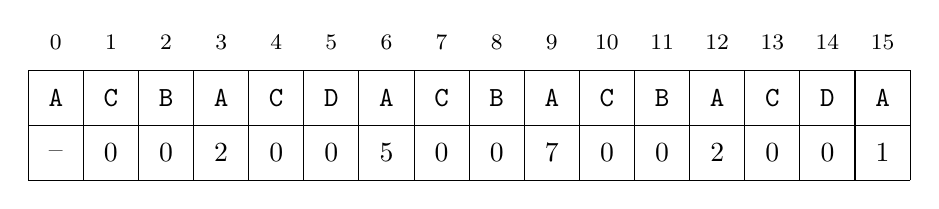
\begin{tikzpicture}[scale=0.7]
\draw (0,0) grid (16,2);

\node at (0.5, 1.5) {\texttt{A}};
\node at (1.5, 1.5) {\texttt{C}};
\node at (2.5, 1.5) {\texttt{B}};
\node at (3.5, 1.5) {\texttt{A}};
\node at (4.5, 1.5) {\texttt{C}};
\node at (5.5, 1.5) {\texttt{D}};
\node at (6.5, 1.5) {\texttt{A}};
\node at (7.5, 1.5) {\texttt{C}};
\node at (8.5, 1.5) {\texttt{B}};
\node at (9.5, 1.5) {\texttt{A}};
\node at (10.5, 1.5) {\texttt{C}};
\node at (11.5, 1.5) {\texttt{B}};
\node at (12.5, 1.5) {\texttt{A}};
\node at (13.5, 1.5) {\texttt{C}};
\node at (14.5, 1.5) {\texttt{D}};
\node at (15.5, 1.5) {\texttt{A}};

\node at (0.5, 0.5) {--};
\node at (1.5, 0.5) {0};
\node at (2.5, 0.5) {0};
\node at (3.5, 0.5) {2};
\node at (4.5, 0.5) {0};
\node at (5.5, 0.5) {0};
\node at (6.5, 0.5) {5};
\node at (7.5, 0.5) {0};
\node at (8.5, 0.5) {0};
\node at (9.5, 0.5) {7};
\node at (10.5, 0.5) {0};
\node at (11.5, 0.5) {0};
\node at (12.5, 0.5) {2};
\node at (13.5, 0.5) {0};
\node at (14.5, 0.5) {0};
\node at (15.5, 0.5) {1};

\footnotesize
\node at (0.5, 2.5) {0};
\node at (1.5, 2.5) {1};
\node at (2.5, 2.5) {2};
\node at (3.5, 2.5) {3};
\node at (4.5, 2.5) {4};
\node at (5.5, 2.5) {5};
\node at (6.5, 2.5) {6};
\node at (7.5, 2.5) {7};
\node at (8.5, 2.5) {8};
\node at (9.5, 2.5) {9};
\node at (10.5, 2.5) {10};
\node at (11.5, 2.5) {11};
\node at (12.5, 2.5) {12};
\node at (13.5, 2.5) {13};
\node at (14.5, 2.5) {14};
\node at (15.5, 2.5) {15};

\end{tikzpicture}
\end{center}

Бұл жағдайда, $\texttt{z}[6]=5$, себебі ұзындығы
5 болатын \texttt{ACBAC} ішжолы \texttt{s} жолының префиксі болады, бірақ ұзындығы 6 болатын \texttt{ACBACB} ішжолы 
\texttt{s} жолының префиксі бола алмайды.

% In this case, for example, $\texttt{z}[6]=5$,
% because the substring \texttt{ACBAC} of length 5
% is a prefix of \texttt{s},
% but the substring \texttt{ACBACB} of length 6
% is not a prefix of \texttt{s}.

\subsubsection*{Алгоритм}

Бұдан әрі біз Z-жиымын $O(n)$ уақытта құрастыратын \key{Z-алгоритм}\footnote{
Z-алгоритмді \cite{gus97} мақаласында үлгімен салғыстырудың танымал қарапайым сызықтық әдісі ретінде ұсынылды, 
бастапқы идея \cite{mai84} тиесілі.}
деп аталатын алгоритмді қарастырамыз. 
Алгоритм Z-жиымның мәндерін 
оған дейін сақталған Z-жиымның мәндерін қолдана отырып, ішжолдардың таңбаларын жеке салыстыра келе, солдан оңға қарай есептейді.

% Next we describe an algorithm,
% called the \key{Z-algorithm}\footnote{The Z-algorithm
% was presented in \cite{gus97} as the simplest known
% method for linear-time pattern matching, and the original idea
% was attributed to \cite{mai84}.},
% that efficiently constructs the Z-array in $O(n)$ time.
% The algorithm calculates the Z-array values
% from left to right by both using information
% already stored in the Z-array and comparing substrings
% character by character.

Z-жиынның мәндерін тиімді есептеу үшін 
алгоритм $\texttt{s}[x \ldots y]$ ішжолы \texttt{s} жолының 
префиксі болатын және $y$ ең максималды болатын
$[x,y]$ аралығын қолдайды. 
$\texttt{s}[0 \ldots y-x]$ және $\texttt{s}[x \ldots y]$
тең болғандықтан, оны $x+1,x+2,\ldots,y$ позицияларының
Z-мәнін есептеуге қолдана аламыз. 

% To efficiently calculate the Z-array values,
% the algorithm maintains a range $[x,y]$ such that
% $\texttt{s}[x \ldots y]$ is a prefix of \texttt{s}
% and $y$ is as large as possible.
% Since we know that $\texttt{s}[0 \ldots y-x]$
% and $\texttt{s}[x \ldots y]$ are equal,
% we can use this information when calculating
% Z-values for positions $x+1,x+2,\ldots,y$.

Әр $k$ позициясына біз алдымен 
$\texttt{z}[k-x]$ мәнін тексереміз.
Егер $k+\texttt{z}[k-x]<y$ болса, онда 
$\texttt{z}[k]=\texttt{z}[k-x]$ екенін білеміз. 
Бірақ $k+\texttt{z}[k-x] \ge y$ болса, 
$\texttt{s}[0 \ldots y-k]$ ішжолы
$\texttt{s}[k \ldots y]$ ішжолына тең болады
және $\texttt{z}[k]$ мәнін анықтау үшін 
ішжолдардың жеке таңбаларын салыстыру керек. 
Дегенмен біз салыстыруды $y-k+1$ және $y+1$ 
позицияларында бастайтын болғандықтан, алгоритм $O(n)$ уақыт жұмыс істейді.

% At each position $k$, we first
% check the value of $\texttt{z}[k-x]$.
% If $k+\texttt{z}[k-x]<y$, we know that $\texttt{z}[k]=\texttt{z}[k-x]$.
% However, if $k+\texttt{z}[k-x] \ge y$,
% $\texttt{s}[0 \ldots y-k]$ equals
% $\texttt{s}[k \ldots y]$, and to determine the
% value of $\texttt{z}[k]$ we need to compare
% the substrings character by character.
% Still, the algorithm works in $O(n)$ time,
% because we start comparing at positions
% $y-k+1$ and $y+1$.

Мысалы, келесі Z-жиымын құрастырайық:
% For example, let us construct the following Z-array:

\begin{center}
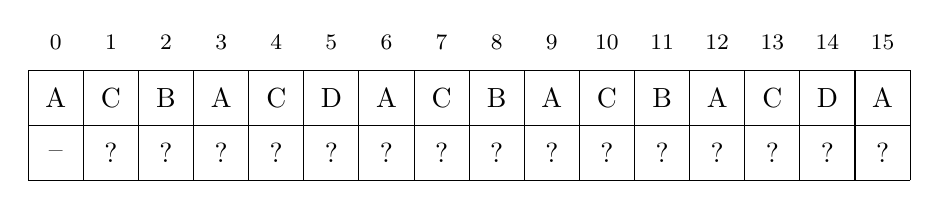
\begin{tikzpicture}[scale=0.7]
\draw (0,0) grid (16,2);

\node at (0.5, 1.5) {A};
\node at (1.5, 1.5) {C};
\node at (2.5, 1.5) {B};
\node at (3.5, 1.5) {A};
\node at (4.5, 1.5) {C};
\node at (5.5, 1.5) {D};
\node at (6.5, 1.5) {A};
\node at (7.5, 1.5) {C};
\node at (8.5, 1.5) {B};
\node at (9.5, 1.5) {A};
\node at (10.5, 1.5) {C};
\node at (11.5, 1.5) {B};
\node at (12.5, 1.5) {A};
\node at (13.5, 1.5) {C};
\node at (14.5, 1.5) {D};
\node at (15.5, 1.5) {A};

\node at (0.5, 0.5) {--};
\node at (1.5, 0.5) {?};
\node at (2.5, 0.5) {?};
\node at (3.5, 0.5) {?};
\node at (4.5, 0.5) {?};
\node at (5.5, 0.5) {?};
\node at (6.5, 0.5) {?};
\node at (7.5, 0.5) {?};
\node at (8.5, 0.5) {?};
\node at (9.5, 0.5) {?};
\node at (10.5, 0.5) {?};
\node at (11.5, 0.5) {?};
\node at (12.5, 0.5) {?};
\node at (13.5, 0.5) {?};
\node at (14.5, 0.5) {?};
\node at (15.5, 0.5) {?};

\footnotesize
\node at (0.5, 2.5) {0};
\node at (1.5, 2.5) {1};
\node at (2.5, 2.5) {2};
\node at (3.5, 2.5) {3};
\node at (4.5, 2.5) {4};
\node at (5.5, 2.5) {5};
\node at (6.5, 2.5) {6};
\node at (7.5, 2.5) {7};
\node at (8.5, 2.5) {8};
\node at (9.5, 2.5) {9};
\node at (10.5, 2.5) {10};
\node at (11.5, 2.5) {11};
\node at (12.5, 2.5) {12};
\node at (13.5, 2.5) {13};
\node at (14.5, 2.5) {14};
\node at (15.5, 2.5) {15};

\end{tikzpicture}
\end{center}

$\texttt{z}[6]=5$ есептеп болғаннан кейін
қазіргі $[x,y]$ аралығы $[6,10]$ тең болады:

% After calculating the value $\texttt{z}[6]=5$,
% the current $[x,y]$ range is $[6,10]$:

\begin{center}
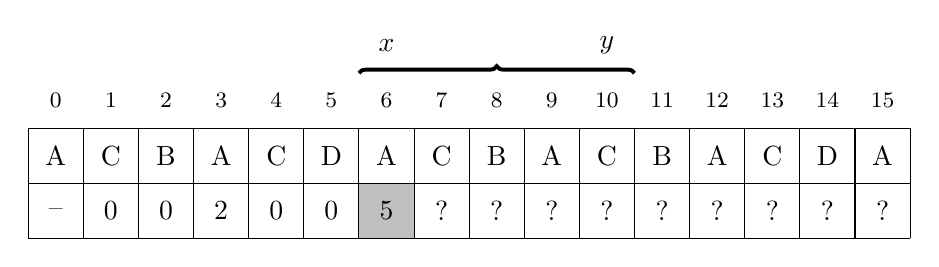
\begin{tikzpicture}[scale=0.7]
\fill[color=lightgray] (6,0) rectangle (7,1);
\draw (0,0) grid (16,2);

\node at (0.5, 1.5) {A};
\node at (1.5, 1.5) {C};
\node at (2.5, 1.5) {B};
\node at (3.5, 1.5) {A};
\node at (4.5, 1.5) {C};
\node at (5.5, 1.5) {D};
\node at (6.5, 1.5) {A};
\node at (7.5, 1.5) {C};
\node at (8.5, 1.5) {B};
\node at (9.5, 1.5) {A};
\node at (10.5, 1.5) {C};
\node at (11.5, 1.5) {B};
\node at (12.5, 1.5) {A};
\node at (13.5, 1.5) {C};
\node at (14.5, 1.5) {D};
\node at (15.5, 1.5) {A};

\node at (0.5, 0.5) {--};
\node at (1.5, 0.5) {0};
\node at (2.5, 0.5) {0};
\node at (3.5, 0.5) {2};
\node at (4.5, 0.5) {0};
\node at (5.5, 0.5) {0};
\node at (6.5, 0.5) {5};
\node at (7.5, 0.5) {?};
\node at (8.5, 0.5) {?};
\node at (9.5, 0.5) {?};
\node at (10.5, 0.5) {?};
\node at (11.5, 0.5) {?};
\node at (12.5, 0.5) {?};
\node at (13.5, 0.5) {?};
\node at (14.5, 0.5) {?};
\node at (15.5, 0.5) {?};

\draw [decoration={brace}, decorate, line width=0.5mm] (6,3.00) -- (11,3.00);

\node at (6.5,3.50) {$x$};
\node at (10.5,3.50) {$y$};


\footnotesize
\node at (0.5, 2.5) {0};
\node at (1.5, 2.5) {1};
\node at (2.5, 2.5) {2};
\node at (3.5, 2.5) {3};
\node at (4.5, 2.5) {4};
\node at (5.5, 2.5) {5};
\node at (6.5, 2.5) {6};
\node at (7.5, 2.5) {7};
\node at (8.5, 2.5) {8};
\node at (9.5, 2.5) {9};
\node at (10.5, 2.5) {10};
\node at (11.5, 2.5) {11};
\node at (12.5, 2.5) {12};
\node at (13.5, 2.5) {13};
\node at (14.5, 2.5) {14};
\node at (15.5, 2.5) {15};

\end{tikzpicture}
\end{center}

Енді келесі Z-жиымның мәндерін 
тиімді есептей аламыз, себебі 
$\texttt{s}[0 \ldots 4]$ мен 
$\texttt{s}[6 \ldots 10]$ тең екенін білеміз. 
Біріншіден, $\texttt{z}[1] = \texttt{z}[2] = 0$ болғандықтан,
$\texttt{z}[7] = \texttt{z}[8] = 0$ екенін де бірден білеміз:

% Now we can calculate
% subsequent Z-array values
% efficiently,
% because we know that
% $\texttt{s}[0 \ldots 4]$ and
% $\texttt{s}[6 \ldots 10]$ are equal.
% First, since $\texttt{z}[1] = \texttt{z}[2] = 0$,
% we immediately know that also
% $\texttt{z}[7] = \texttt{z}[8] = 0$:

\begin{center}
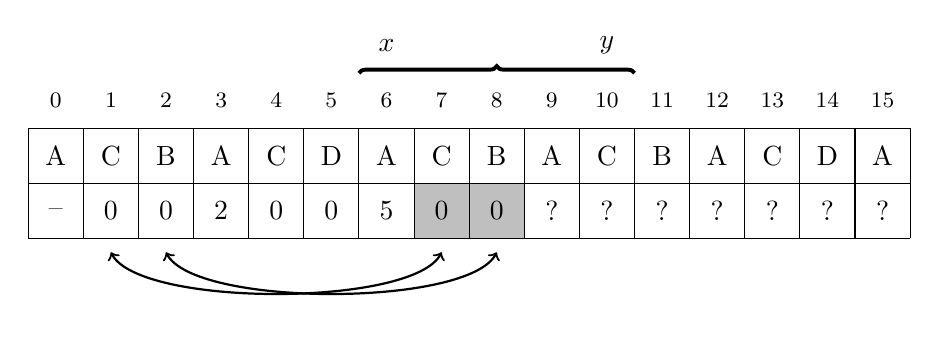
\begin{tikzpicture}[scale=0.7]
\fill[color=lightgray] (7,0) rectangle (9,1);
\draw (0,0) grid (16,2);

\node at (0.5, 1.5) {A};
\node at (1.5, 1.5) {C};
\node at (2.5, 1.5) {B};
\node at (3.5, 1.5) {A};
\node at (4.5, 1.5) {C};
\node at (5.5, 1.5) {D};
\node at (6.5, 1.5) {A};
\node at (7.5, 1.5) {C};
\node at (8.5, 1.5) {B};
\node at (9.5, 1.5) {A};
\node at (10.5, 1.5) {C};
\node at (11.5, 1.5) {B};
\node at (12.5, 1.5) {A};
\node at (13.5, 1.5) {C};
\node at (14.5, 1.5) {D};
\node at (15.5, 1.5) {A};

\node at (0.5, 0.5) {--};
\node at (1.5, 0.5) {0};
\node at (2.5, 0.5) {0};
\node at (3.5, 0.5) {2};
\node at (4.5, 0.5) {0};
\node at (5.5, 0.5) {0};
\node at (6.5, 0.5) {5};
\node at (7.5, 0.5) {0};
\node at (8.5, 0.5) {0};
\node at (9.5, 0.5) {?};
\node at (10.5, 0.5) {?};
\node at (11.5, 0.5) {?};
\node at (12.5, 0.5) {?};
\node at (13.5, 0.5) {?};
\node at (14.5, 0.5) {?};
\node at (15.5, 0.5) {?};


\draw [decoration={brace}, decorate, line width=0.5mm] (6,3.00) -- (11,3.00);

\node at (6.5,3.50) {$x$};
\node at (10.5,3.50) {$y$};


\footnotesize
\node at (0.5, 2.5) {0};
\node at (1.5, 2.5) {1};
\node at (2.5, 2.5) {2};
\node at (3.5, 2.5) {3};
\node at (4.5, 2.5) {4};
\node at (5.5, 2.5) {5};
\node at (6.5, 2.5) {6};
\node at (7.5, 2.5) {7};
\node at (8.5, 2.5) {8};
\node at (9.5, 2.5) {9};
\node at (10.5, 2.5) {10};
\node at (11.5, 2.5) {11};
\node at (12.5, 2.5) {12};
\node at (13.5, 2.5) {13};
\node at (14.5, 2.5) {14};
\node at (15.5, 2.5) {15};


\draw[thick,<->] (7.5,-0.25) .. controls (7,-1.25) and (2,-1.25) .. (1.5,-0.25);
\draw[thick,<->] (8.5,-0.25) .. controls (8,-1.25) and (3,-1.25) .. (2.5,-0.25);
\end{tikzpicture}
\end{center}

Кейін $\texttt{z}[3]=2$ болғандықтан, $\texttt{z}[9] \ge 2$ екенін білеміз:

% Then, since $\texttt{z}[3]=2$, we know that $\texttt{z}[9] \ge 2$:

\begin{center}
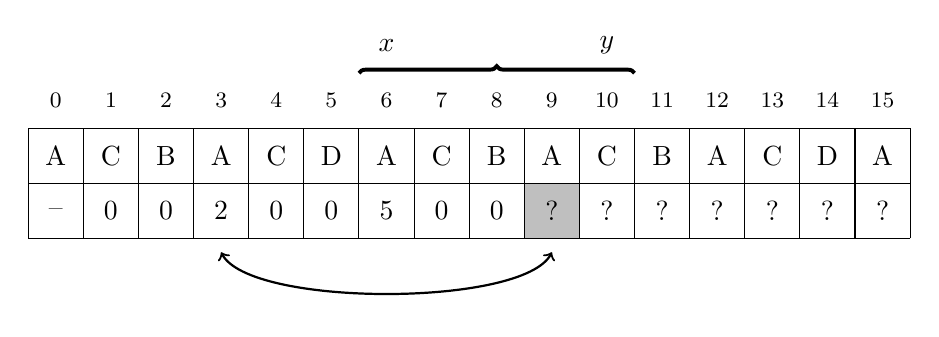
\begin{tikzpicture}[scale=0.7]
\fill[color=lightgray] (9,0) rectangle (10,1);
\draw (0,0) grid (16,2);

\node at (0.5, 1.5) {A};
\node at (1.5, 1.5) {C};
\node at (2.5, 1.5) {B};
\node at (3.5, 1.5) {A};
\node at (4.5, 1.5) {C};
\node at (5.5, 1.5) {D};
\node at (6.5, 1.5) {A};
\node at (7.5, 1.5) {C};
\node at (8.5, 1.5) {B};
\node at (9.5, 1.5) {A};
\node at (10.5, 1.5) {C};
\node at (11.5, 1.5) {B};
\node at (12.5, 1.5) {A};
\node at (13.5, 1.5) {C};
\node at (14.5, 1.5) {D};
\node at (15.5, 1.5) {A};

\node at (0.5, 0.5) {--};
\node at (1.5, 0.5) {0};
\node at (2.5, 0.5) {0};
\node at (3.5, 0.5) {2};
\node at (4.5, 0.5) {0};
\node at (5.5, 0.5) {0};
\node at (6.5, 0.5) {5};
\node at (7.5, 0.5) {0};
\node at (8.5, 0.5) {0};
\node at (9.5, 0.5) {?};
\node at (10.5, 0.5) {?};
\node at (11.5, 0.5) {?};
\node at (12.5, 0.5) {?};
\node at (13.5, 0.5) {?};
\node at (14.5, 0.5) {?};
\node at (15.5, 0.5) {?};

\draw [decoration={brace}, decorate, line width=0.5mm] (6,3.00) -- (11,3.00);

\node at (6.5,3.50) {$x$};
\node at (10.5,3.50) {$y$};


\footnotesize
\node at (0.5, 2.5) {0};
\node at (1.5, 2.5) {1};
\node at (2.5, 2.5) {2};
\node at (3.5, 2.5) {3};
\node at (4.5, 2.5) {4};
\node at (5.5, 2.5) {5};
\node at (6.5, 2.5) {6};
\node at (7.5, 2.5) {7};
\node at (8.5, 2.5) {8};
\node at (9.5, 2.5) {9};
\node at (10.5, 2.5) {10};
\node at (11.5, 2.5) {11};
\node at (12.5, 2.5) {12};
\node at (13.5, 2.5) {13};
\node at (14.5, 2.5) {14};
\node at (15.5, 2.5) {15};

\draw[thick,<->] (9.5,-0.25) .. controls (9,-1.25) and (4,-1.25) .. (3.5,-0.25);
\end{tikzpicture}
\end{center}

Дегенмен 10-позициядан кейінгі жол жайында еш ақпарат болмағандықтан,
ішжолдардың таңбаларын жеке салыстыруға тура келеді:

% However, we have no information about the string
% after position 10, so we need to compare the substrings
% character by character:

\begin{center}
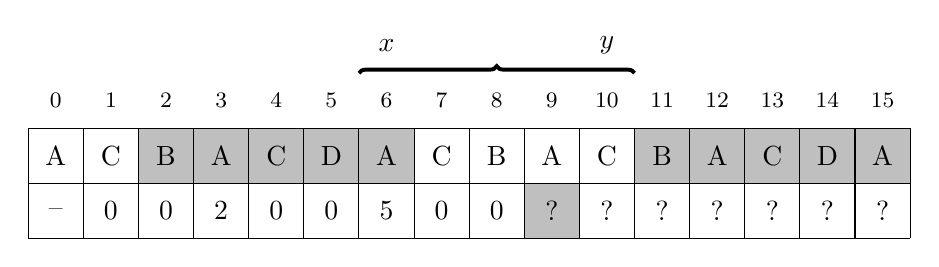
\begin{tikzpicture}[scale=0.7]
\fill[color=lightgray] (9,0) rectangle (10,1);
\fill[color=lightgray] (2,1) rectangle (7,2);
\fill[color=lightgray] (11,1) rectangle (16,2);


\draw (0,0) grid (16,2);

\node at (0.5, 1.5) {A};
\node at (1.5, 1.5) {C};
\node at (2.5, 1.5) {B};
\node at (3.5, 1.5) {A};
\node at (4.5, 1.5) {C};
\node at (5.5, 1.5) {D};
\node at (6.5, 1.5) {A};
\node at (7.5, 1.5) {C};
\node at (8.5, 1.5) {B};
\node at (9.5, 1.5) {A};
\node at (10.5, 1.5) {C};
\node at (11.5, 1.5) {B};
\node at (12.5, 1.5) {A};
\node at (13.5, 1.5) {C};
\node at (14.5, 1.5) {D};
\node at (15.5, 1.5) {A};

\node at (0.5, 0.5) {--};
\node at (1.5, 0.5) {0};
\node at (2.5, 0.5) {0};
\node at (3.5, 0.5) {2};
\node at (4.5, 0.5) {0};
\node at (5.5, 0.5) {0};
\node at (6.5, 0.5) {5};
\node at (7.5, 0.5) {0};
\node at (8.5, 0.5) {0};
\node at (9.5, 0.5) {?};
\node at (10.5, 0.5) {?};
\node at (11.5, 0.5) {?};
\node at (12.5, 0.5) {?};
\node at (13.5, 0.5) {?};
\node at (14.5, 0.5) {?};
\node at (15.5, 0.5) {?};

\draw [decoration={brace}, decorate, line width=0.5mm] (6,3.00) -- (11,3.00);

\node at (6.5,3.50) {$x$};
\node at (10.5,3.50) {$y$};


\footnotesize
\node at (0.5, 2.5) {0};
\node at (1.5, 2.5) {1};
\node at (2.5, 2.5) {2};
\node at (3.5, 2.5) {3};
\node at (4.5, 2.5) {4};
\node at (5.5, 2.5) {5};
\node at (6.5, 2.5) {6};
\node at (7.5, 2.5) {7};
\node at (8.5, 2.5) {8};
\node at (9.5, 2.5) {9};
\node at (10.5, 2.5) {10};
\node at (11.5, 2.5) {11};
\node at (12.5, 2.5) {12};
\node at (13.5, 2.5) {13};
\node at (14.5, 2.5) {14};
\node at (15.5, 2.5) {15};

%\draw[thick,<->] (11.5,-0.25) .. controls (11,-1.25) and (3,-1.25) .. (2.5,-0.25);
\end{tikzpicture}
\end{center}

$\texttt{z}[9]=7$ екені белгілі болған соң,
жаңа $[x,y]$ аралығы $[9,15]$ аралығына тең болды:

% It turns out that $\texttt{z}[9]=7$,
% so the new $[x,y]$ range is $[9,15]$:

\begin{center}
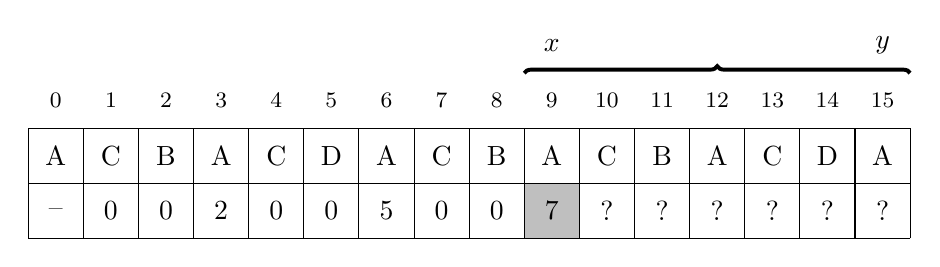
\begin{tikzpicture}[scale=0.7]
\fill[color=lightgray] (9,0) rectangle (10,1);
\draw (0,0) grid (16,2);

\node at (0.5, 1.5) {A};
\node at (1.5, 1.5) {C};
\node at (2.5, 1.5) {B};
\node at (3.5, 1.5) {A};
\node at (4.5, 1.5) {C};
\node at (5.5, 1.5) {D};
\node at (6.5, 1.5) {A};
\node at (7.5, 1.5) {C};
\node at (8.5, 1.5) {B};
\node at (9.5, 1.5) {A};
\node at (10.5, 1.5) {C};
\node at (11.5, 1.5) {B};
\node at (12.5, 1.5) {A};
\node at (13.5, 1.5) {C};
\node at (14.5, 1.5) {D};
\node at (15.5, 1.5) {A};

\node at (0.5, 0.5) {--};
\node at (1.5, 0.5) {0};
\node at (2.5, 0.5) {0};
\node at (3.5, 0.5) {2};
\node at (4.5, 0.5) {0};
\node at (5.5, 0.5) {0};
\node at (6.5, 0.5) {5};
\node at (7.5, 0.5) {0};
\node at (8.5, 0.5) {0};
\node at (9.5, 0.5) {7};
\node at (10.5, 0.5) {?};
\node at (11.5, 0.5) {?};
\node at (12.5, 0.5) {?};
\node at (13.5, 0.5) {?};
\node at (14.5, 0.5) {?};
\node at (15.5, 0.5) {?};

\draw [decoration={brace}, decorate, line width=0.5mm] (9,3.00) -- (16,3.00);

\node at (9.5,3.50) {$x$};
\node at (15.5,3.50) {$y$};


\footnotesize
\node at (0.5, 2.5) {0};
\node at (1.5, 2.5) {1};
\node at (2.5, 2.5) {2};
\node at (3.5, 2.5) {3};
\node at (4.5, 2.5) {4};
\node at (5.5, 2.5) {5};
\node at (6.5, 2.5) {6};
\node at (7.5, 2.5) {7};
\node at (8.5, 2.5) {8};
\node at (9.5, 2.5) {9};
\node at (10.5, 2.5) {10};
\node at (11.5, 2.5) {11};
\node at (12.5, 2.5) {12};
\node at (13.5, 2.5) {13};
\node at (14.5, 2.5) {14};
\node at (15.5, 2.5) {15};

% \draw[thick,<->] (9.5,-0.25) .. controls (9,-1.25) and (4,-1.25) .. (3.5,-0.25);
\end{tikzpicture}
\end{center}

Одан кейін барлық Z-жиынның мәндерін 
Z-жиымда оған дейін сақталған ақпараттар арқылы
анықтауымызға болады:

% After this, all the remaining Z-array values
% can be determined by using the information
% already stored in the Z-array:

\begin{center}
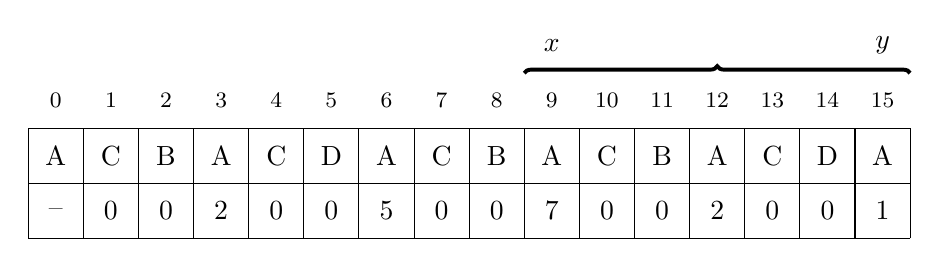
\begin{tikzpicture}[scale=0.7]
\draw (0,0) grid (16,2);

\node at (0.5, 1.5) {A};
\node at (1.5, 1.5) {C};
\node at (2.5, 1.5) {B};
\node at (3.5, 1.5) {A};
\node at (4.5, 1.5) {C};
\node at (5.5, 1.5) {D};
\node at (6.5, 1.5) {A};
\node at (7.5, 1.5) {C};
\node at (8.5, 1.5) {B};
\node at (9.5, 1.5) {A};
\node at (10.5, 1.5) {C};
\node at (11.5, 1.5) {B};
\node at (12.5, 1.5) {A};
\node at (13.5, 1.5) {C};
\node at (14.5, 1.5) {D};
\node at (15.5, 1.5) {A};

\node at (0.5, 0.5) {--};
\node at (1.5, 0.5) {0};
\node at (2.5, 0.5) {0};
\node at (3.5, 0.5) {2};
\node at (4.5, 0.5) {0};
\node at (5.5, 0.5) {0};
\node at (6.5, 0.5) {5};
\node at (7.5, 0.5) {0};
\node at (8.5, 0.5) {0};
\node at (9.5, 0.5) {7};
\node at (10.5, 0.5) {0};
\node at (11.5, 0.5) {0};
\node at (12.5, 0.5) {2};
\node at (13.5, 0.5) {0};
\node at (14.5, 0.5) {0};
\node at (15.5, 0.5) {1};

\draw [decoration={brace}, decorate, line width=0.5mm] (9,3.00) -- (16,3.00);

\node at (9.5,3.50) {$x$};
\node at (15.5,3.50) {$y$};


\footnotesize
\node at (0.5, 2.5) {0};
\node at (1.5, 2.5) {1};
\node at (2.5, 2.5) {2};
\node at (3.5, 2.5) {3};
\node at (4.5, 2.5) {4};
\node at (5.5, 2.5) {5};
\node at (6.5, 2.5) {6};
\node at (7.5, 2.5) {7};
\node at (8.5, 2.5) {8};
\node at (9.5, 2.5) {9};
\node at (10.5, 2.5) {10};
\node at (11.5, 2.5) {11};
\node at (12.5, 2.5) {12};
\node at (13.5, 2.5) {13};
\node at (14.5, 2.5) {14};
\node at (15.5, 2.5) {15};

\end{tikzpicture}
\end{center}

\subsubsection{Қолданысы}

Хэшті немесе Z-алгоритмін қолдану әдетте талғамға байланысты болады.
Хэшке қарағанда Z-алгоритмі әрдайым тиімді жұмыс істейді және
қақтығыс болу ықтималдығы жоқ. Дегенмен
Z-алгоримтін жазу қиынырақ және кейбір есептерді тек 
хэш арқылы шығаруға болады. 

% It is often a matter of taste whether to use
% string hashing or the Z-algorithm.
% Unlike hashing, the Z-algorithm always works
% and there is no risk for collisions.
% On the other hand, the Z-algorithm is more difficult
% to implement and some problems can only be solved
% using hashing.

Мысал ретінде үлгі салғыстыру есебін
қайтадан қарастырайық. 
Есепте $p$ үлгісінің
қайда кездесетінін табу керек. Біз бұл есепті осыған дейін хэш арқылы тиімді шығардық, дегенмен Z-алгоритмі есепті 
шешудің басқа жолын ұсынады. 

% As an example, consider again
% the pattern matching problem,
% where our task is to find the occurrences
% of a pattern $p$ in a string $s$.
% We already solved this problem efficiently
% using string hashing, but the Z-algorithm
% provides another way to solve the problem.

Жол өңдеудегі әдеттегі идея 
арнайы таңбамен ажыратылған бірнеше жолдардан тұратын
жолды құрастыруға негізделеді. Бұл есепте $p$\texttt{\#}$s$ жолын
құрастыра аламыз, мұнда $p$ мен $s$ жолдарда
кездеспейтін \texttt{\#} арнайы таңбасы арқылы ажыратылған. 
$p$\texttt{\#}$s$ жолының Z–жиымы $p$-ның $s$-те қай позицияларда 
кездесетінін хабарлайды: олар -- мәні $p$ ұзындығы болатын позициялар.

% A usual idea in string processing is to
% construct a string that consists of
% multiple strings separated by special characters.
% In this problem, we can construct a string
% $p$\texttt{\#}$s$,
% where $p$ and $s$ are separated by a special
% character \texttt{\#} that does not occur
% in the strings.
% The Z-array of $p$\texttt{\#}$s$ tells us the positions
% where $p$ occurs in $s$,
% because such positions contain the length of $p$.

Мысалы, егер $s=$\texttt{HATTIVATTI} және $p=$\texttt{ATT} болса,
Z-жиымы келесідей болады:

% For example, if $s=$\text 
\begin{center}
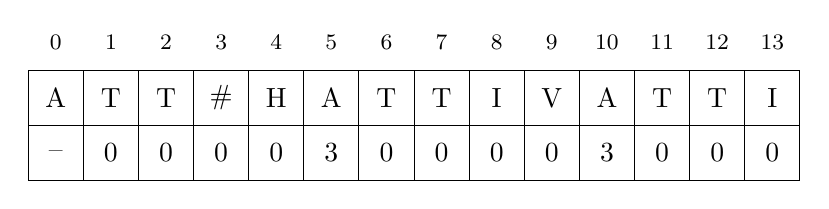
\begin{tikzpicture}[scale=0.7]
\draw (0,0) grid (14,2);

\node at (0.5, 1.5) {A};
\node at (1.5, 1.5) {T};
\node at (2.5, 1.5) {T};
\node at (3.5, 1.5) {\#};
\node at (4.5, 1.5) {H};
\node at (5.5, 1.5) {A};
\node at (6.5, 1.5) {T};
\node at (7.5, 1.5) {T};
\node at (8.5, 1.5) {I};
\node at (9.5, 1.5) {V};
\node at (10.5, 1.5) {A};
\node at (11.5, 1.5) {T};
\node at (12.5, 1.5) {T};
\node at (13.5, 1.5) {I};

\node at (0.5, 0.5) {--};
\node at (1.5, 0.5) {0};
\node at (2.5, 0.5) {0};
\node at (3.5, 0.5) {0};
\node at (4.5, 0.5) {0};
\node at (5.5, 0.5) {3};
\node at (6.5, 0.5) {0};
\node at (7.5, 0.5) {0};
\node at (8.5, 0.5) {0};
\node at (9.5, 0.5) {0};
\node at (10.5, 0.5) {3};
\node at (11.5, 0.5) {0};
\node at (12.5, 0.5) {0};
\node at (13.5, 0.5) {0};

\footnotesize
\node at (0.5, 2.5) {0};
\node at (1.5, 2.5) {1};
\node at (2.5, 2.5) {2};
\node at (3.5, 2.5) {3};
\node at (4.5, 2.5) {4};
\node at (5.5, 2.5) {5};
\node at (6.5, 2.5) {6};
\node at (7.5, 2.5) {7};
\node at (8.5, 2.5) {8};
\node at (9.5, 2.5) {9};
\node at (10.5, 2.5) {10};
\node at (11.5, 2.5) {11};
\node at (12.5, 2.5) {12};
\node at (13.5, 2.5) {13};
\end{tikzpicture}
\end{center}

5 және 10-позициядағы элементтердің мәндері -- 3,
демек \texttt{ATT} үлгісі \texttt{HATTIVATTI} жолындағы
сәйкес позицияларда кездеседі. 

% The positions 5 and 10 contain the value 3,
% which means that the pattern \texttt{ATT}
% occurs in the corresponding positions
% of \texttt{HATTIVATTI}.

Z-жиымды құрастырып, оның мәндерінен өтіп шығу жеткілікті болғандықтан нәтижелік алгоритмде сызықтық уақытша күрделігі сақталады.

% The time complexity of the resulting algorithm
% is linear, because it suffices to construct
% the Z-array and go through its values.

\subsubsection{Коды}

Төменде Z-жиымына сәйкес векторды қайтаратын Z-алгоритмінің қысқа 
коды берілген:

% Here is a short implementation of the Z-algorithm
% that returns a vector that corresponds to the Z-array.

\begin{lstlisting}
vector<int> z(string s) {
    int n = s.size();
    vector<int> z(n);
    int x = 0, y = 0;
    for (int i = 1; i < n; i++) {
        z[i] = max(0,min(z[i-x],y-i+1));
        while (i+z[i] < n && s[z[i]] == s[i+z[i]]) {
            x = i; y = i+z[i]; z[i]++;
        }
    }
    return z;
}
\end{lstlisting}